\documentclass[a4paper, 10pt, final, garamond]{book}
\usepackage{cours-preambule}

\makeatletter
\renewcommand{\@chapapp}{Contr\^ole de connaissances}
\makeatother

\toggletrue{student}
\HideSolutionstrue

\begin{document}
\setcounter{chapter}{-1}

\chapter{Rentrée, unités, mesure et optique}

\begin{center}
	\Large \textit{Calculatrice autorisée.}
\end{center}

\begin{enumerate}[label=\sqenumi]
	\nitem{1} Citer, sans détailler, les trois astuces pour reprendre le contrôle
	sur son utilisation du téléphone.
	\smallbreak
	\wsw{
		Restriction du temps, contrainte physique et contrainte catégorique.
	}
	\nitem{2}
	Donner, par analyse dimensionnelle, la période $T$ des oscillations d'un
	pendule simple sans facteur multiplicatif.
	\smallbreak
	\wsw{
		Les variables possibles sont
		$\ell$, $g$ et $m$~; ainsi, il nous faudrait avoir
	}
	\smallbreak
	\begin{isd}
		\wsw{
			\begin{gather*}
				T = \ell^{\alpha}g^{\beta}m^{\gamma}
				\\\Lra
				[T] = [\ell]^{\alpha}[g]^{\beta}[m]^{\gamma}
				\\\Lra
				\si{s} = \si{m^{\alpha}.m^{\beta}.s^{-2\beta}.kg^{\gamma}}
				\\\Lra
				\left\{
				\begin{array}{rcl}
					\si{s} & = & \si{s}^{-2 \beta}
					\\
					1      & = & \si{m}^{\alpha+\beta}
					\\
					1      & = & \si{kg}^{\gamma}
				\end{array}
				\right.
				\Lra
				\left\{
				\begin{array}{rcl}
					\beta  & = & - \frac{1}{2}
					\\
					\alpha & = & \frac{1}{2}
					\\
					\gamma & = & 0
				\end{array}
				\right.
			\end{gather*}
		}
		\tcblower
		\wsw{
			Autrement dit, on aurait tendance à écrire
			\[
				\boxed{T = \sqrt{\frac{\ell}{g}}}
			\]
			Ce qui serait effectivement homogène~! Mais pourtant faux… L'étude
			complète du système donne un \textbf{facteur} $\mathbf{2\pi}$ avant la
			racine.
		}
	\end{isd}
	\vspace*{-20pt}
	\nitem{2} Comment valider une régression linéaire~? Deux éléments sont
	attendus, ainsi que deux schémas grossiers représentatifs de régressions.
	\smallbreak
	\begin{isd}[righthand ratio=.4]
		\wsw{
			Par étude visuelle~: les données doivent décrire une droite et être
			suffisamment proche de la régression~; par étude numérique~: le coeffcient de
			corrélation doit être supérieur à \num{0.99}.
			\smallbreak
			À droite, le premier cas est valide. Le second non.
		}
		\tcblower
		\begin{center}
			\switch{
				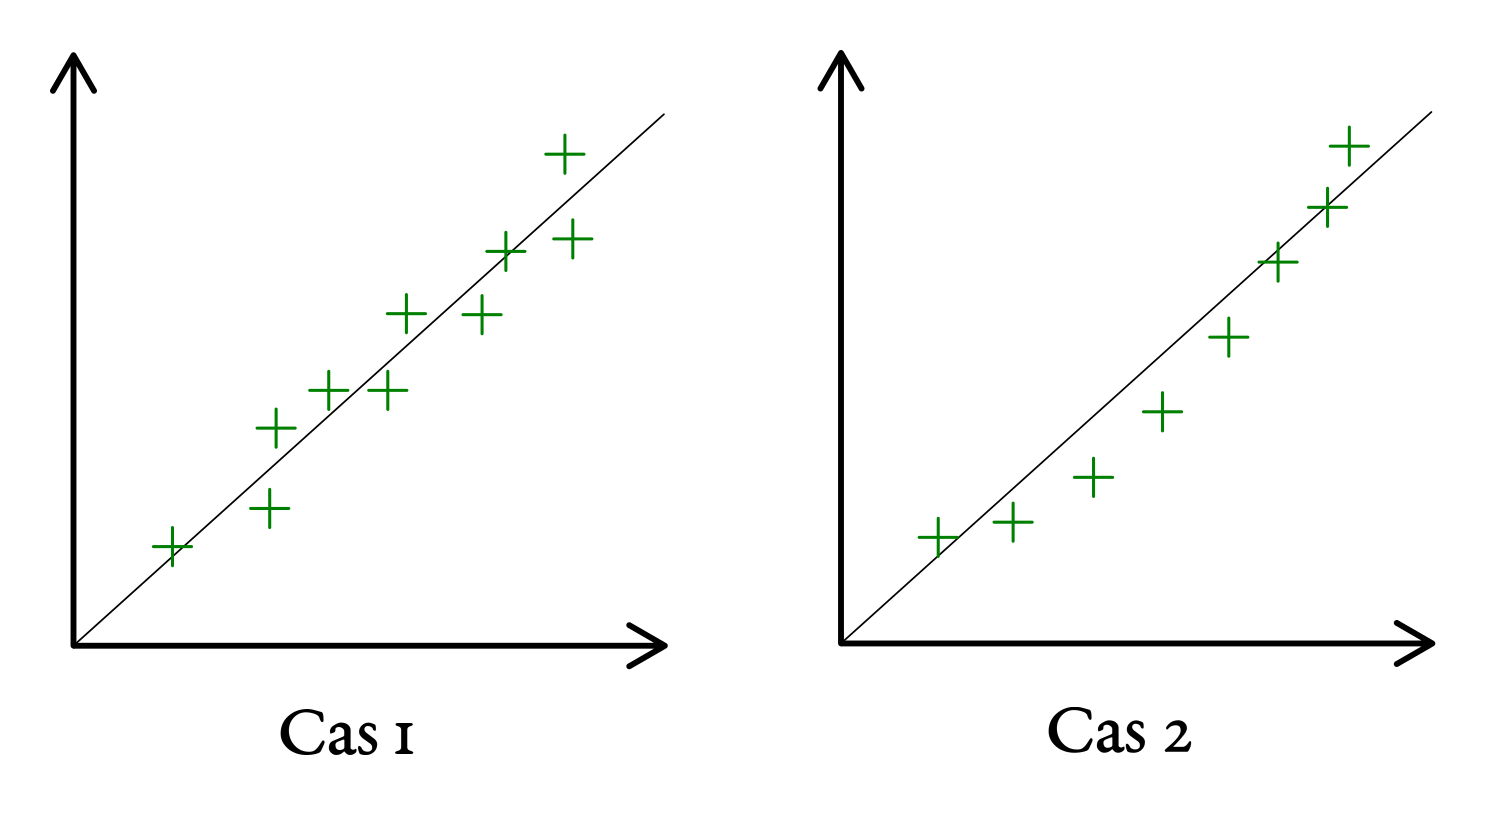
\includegraphics[width=\linewidth, draft=true]{reglin_nl}
				% \captionof{figure}{}
			}{
				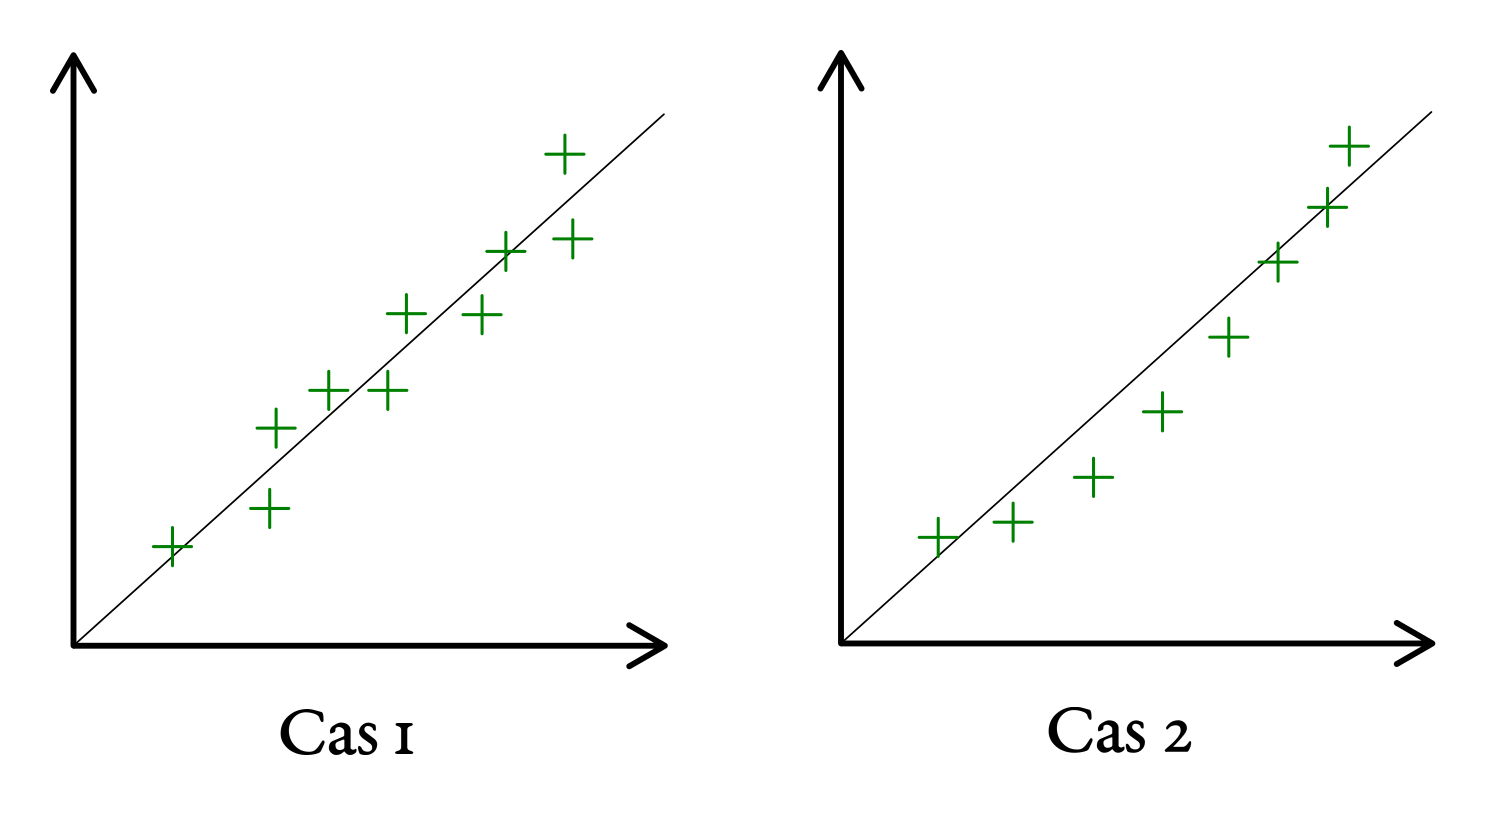
\includegraphics[width=\linewidth]{reglin_nl}
				% \captionof{figure}{Le cas 1 est validé. Le second non.}
			}
		\end{center}
		\vspace*{-20pt}
	\end{isd}
	% \nitem{4} La tension et l'intensité sont mesurées au travers d'une
	% résistance de $R= \SI{1}{k\Omega}$ d'après le constructeur.
	% \begin{center}
	% 	\begin{tabular}{ l  c  c  c  c  c  c }
	% 		\toprule
	% 		$I$ (en A)  & \num{0,010} & \num{0,020} & \num{0,030} & \num{0,040} &
	% 		\num{0,050} & \num{0,060}                                             \\
	% 		$U$ (en V)  & \num{10,0}  & \num{15,0}  & \num{26.0}  & \num{45.0}  &
	% 		\num{65.0}  & \num{100.0}                                             \\
	% 		\bottomrule
	% 	\end{tabular}
	% \end{center}
	% Les données suivent-elles bien la loi d’\textsc{Ohm}~? Vous répondrez
	% textuellement à gauche et représenterez \textbf{grossièrement} (pas de
	% valeur numérique sur les axes) à droite.
	% \smallbreak
	% \begin{isd}
	% 	\wsw{
	% 		On trouve le graphique ci-contre. On contrôle
	% 		la validité~:
	% 		\begin{enumerate}
	% 			\item Visuellement, les données ne suivent pas une droite.
	% 			\item L'ordonnée à l'origine est de \SI{-18}{V} pour une
	% 			      fonction supposée linéaire.
	% 			\item Le coefficient directeur est de $\SI{1.8}{k\Omega}$ pour
	% 			      une valeur normalement proche de $\SI{1}{k\Omega}$, soit un
	% 			      écart relatif de 80\%
	% 			\item Le coeffcient de corrélation est $r^{2} = \num{0.92}$.
	% 		\end{enumerate}
	% 		La régression n'est donc \textbf{pas validée}.
	% 	}
	% 	\tcblower
	% 	\begin{center}
	% 		\switch{
	% 			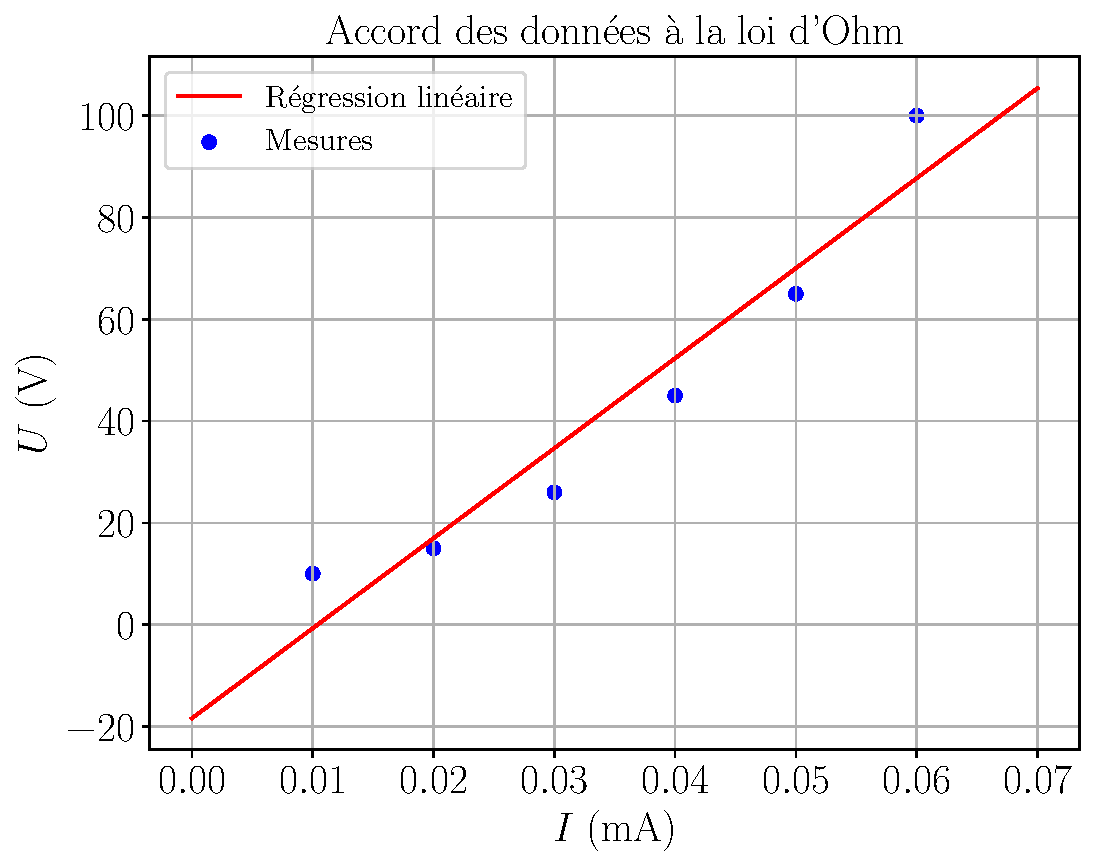
\includegraphics[width=.7\linewidth, draft=true]{reglin}
	% 		}{
	% 			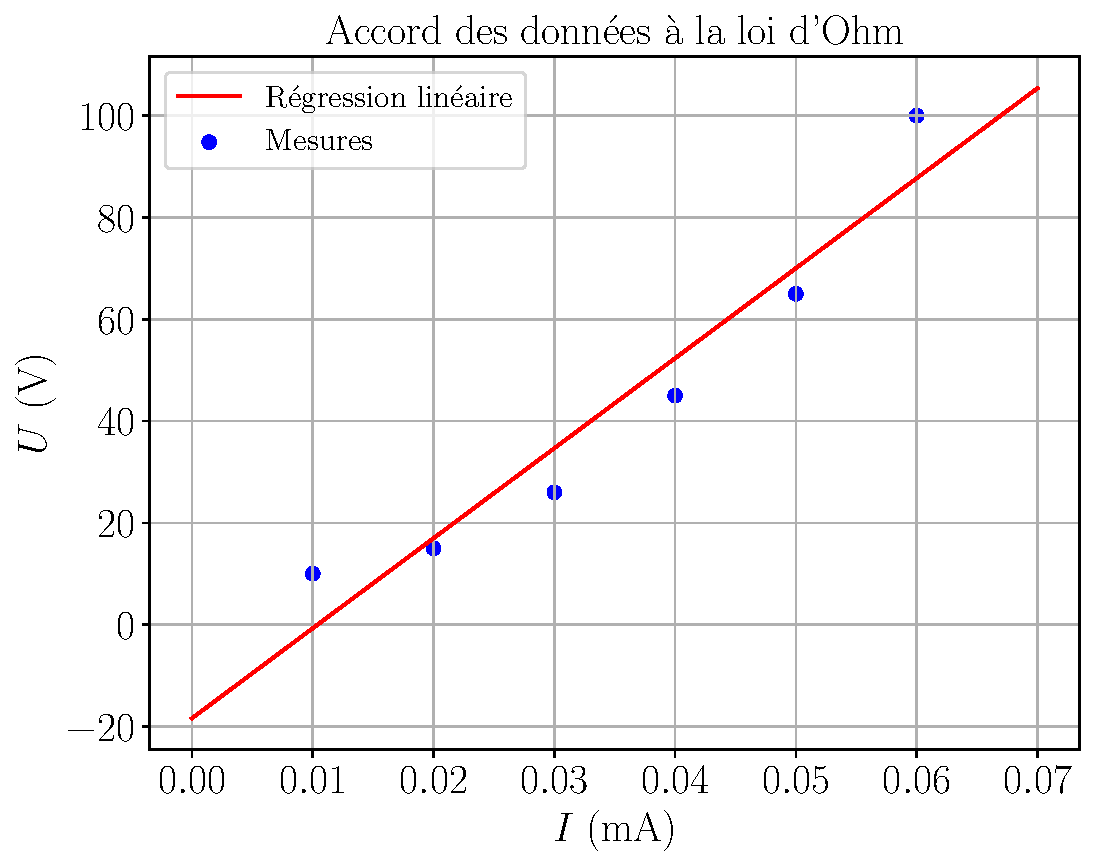
\includegraphics[width=.7\linewidth]{reglin}
	% 		}
	% 		\captionof{figure}{Représentation grossière de la régression.}
	% 	\end{center}
	% \end{isd}
	\nitem{2} Corriger la présentation des valeurs suivantes, indiquer leur nombre de
	chiffres significatifs et calculer leurs incertitudes relatives $u_r$~:
	\[
		\lambda = \SI{589.0\pm11}{nm}
		\qquad
		t = \SI{0.473 \pm 0.122}{s}
		\qquad
		V = (14 \pm \num{0.0015})\,\si{mL}
	\]
	\wsw{
		On trouve
		\[
			\lambda = \SI{589\pm11}{nm}
			\qquad
			t = \SI{0.47 \pm 0.12}{s}
			\qquad
			V = \SI{14.0000 \pm 0.0015}{mL}
		\]
		avec respectivement 3, 2 et 6 chiffres significatifs. Pour les $u_r$, on trouve
		\[
			u_r(\lambda) = 1.9\%
			\qquad
			u_r(t) = 26\%
			\qquad
			u_r(V) = \num{0.011}\%
		\]
	}
	\vspace*{-20pt}
	\nitem{2}
	Un laser rouge émet un rayonnement de longueur d'onde dans le vide
	$\lambda_0 = \SI{633}{nm}$. Déterminer sa longueur d'onde $\lambda$ dans du
	verre, d'indice optique $n = \num{1.5}$. Sa couleur change-t-elle~?
	\smallbreak
	\begin{isd}[lefthand ratio=.35]
		\wsw{
			On a
			\begin{gather*}
				\boxed{\lambda = \frac{\lambda_0}{n}}
				\qav
				\left\{
				\begin{array}{rcl}
					\lambda_0 & = & \SI{633}{nm}
					\\
					n         & = & \num{1.5}
				\end{array}
				\right.\\
				\mathrm{A.N.~:}\enskip
				\xul{
					\lambda = \SI{422}{nm}
				}
			\end{gather*}
		}
		\vspace*{-20pt}
		\tcblower
		\wsw{
			Cependant, \textbf{sa couleur ne change pas} puis qu'\xul{une onde est
				caracétrisée par sa fréquence}, qui ne change pas.
		}
		\vspace*{-20pt}
	\end{isd}
	\nitem{1} Donner les trois propriétés d'un rayon lumineux.
	\smallbreak
	\wsw{
		Propagation rectligne dans un milieu TLHI, indépendance des rayons lumineux,
		retour inverse dans un milieu TLI.
	}
\end{enumerate}

\end{document}
